\documentclass[11pt,a4paper]{article}

% ---------------------------------------------------------------------------
% Fonts (XeLaTeX) — Segoe UI, matching the web app / slide deck
% ---------------------------------------------------------------------------
\usepackage{fontspec}
\setmainfont{Segoe UI}
\setsansfont{Segoe UI}

\usepackage[margin=2.3cm,top=2.6cm,bottom=2.8cm]{geometry}
\usepackage{amsmath,amssymb}
\usepackage{graphicx}
\usepackage{enumitem}
\usepackage{tikz}
\usepackage{xcolor}
\usepackage{titlesec}
\usepackage{fancyhdr}
\usepackage{hyperref}
\usepackage{booktabs}

% ---------------------------------------------------------------------------
% Palette — same as frontend/src/styles/variables.css / the slide deck
% ---------------------------------------------------------------------------
\definecolor{bgPrimary}{HTML}{7678ED}
\definecolor{cardBg}{HTML}{221F5B}
\definecolor{formulaBg}{HTML}{171449}
\definecolor{goldAccent}{HTML}{C98A00}   % darkened slightly for AA contrast on white
\definecolor{goldAccentBright}{HTML}{F7B801}
\definecolor{orangeAccent}{HTML}{D9740A}
\definecolor{redAccent}{HTML}{E5495A}
\definecolor{blueAccent}{HTML}{2E7BD6}
\definecolor{textDark}{HTML}{1B1830}
\definecolor{textMutedDark}{HTML}{5B5780}

\hypersetup{
  colorlinks=true, linkcolor=orangeAccent, citecolor=orangeAccent,
  urlcolor=blueAccent,
  pdftitle={DSP Studio --- Algorithm Reference},
  pdfauthor={Md Mostakim; Samiul Basir Adry}
}

% Section styling
\titleformat{\section}
  {\normalfont\Large\bfseries\color{cardBg}}
  {\thesection}{0.6em}{}
\titleformat{\subsection}
  {\normalfont\large\bfseries\color{orangeAccent}}
  {\thesubsection}{0.6em}{}
\titlespacing*{\section}{0pt}{1.6em}{0.8em}
\titlespacing*{\subsection}{0pt}{1.2em}{0.5em}

\pagestyle{fancy}
\fancyhf{}
\renewcommand{\headrulewidth}{0pt}
\fancyfoot[L]{\small\color{textMutedDark} DSP Studio --- Algorithm Reference}
\fancyfoot[R]{\small\color{textMutedDark}\thepage}

% Numbered algorithm-step list
\setlist[enumerate,1]{itemsep=3pt,topsep=4pt,leftmargin=*,
  label=\textcolor{orangeAccent}{\textbf{\arabic*.}}}

% A dark "formula card", same visual language as the slide deck, on a
% white page.
\newcommand{\FormulaBox}[1]{%
  \begin{center}
  \begin{tikzpicture}
    \node[rounded corners=6pt, fill=formulaBg, text=white, inner sep=10pt,
          text width=0.86\linewidth, align=center] {#1};
  \end{tikzpicture}
  \end{center}
}

\newcommand{\AlgoHead}{\noindent\textbf{\color{cardBg}Algorithm}\par\vspace{2pt}}
\newcommand{\WhatHead}{\noindent\textbf{\color{cardBg}What it does}\par\vspace{2pt}}
\newcommand{\NoteHead}{\noindent\textbf{\color{cardBg}Implementation note}\par\vspace{2pt}}

\graphicspath{{figures/}}

\title{\vspace{-2cm}}
\date{}

\begin{document}

% ============================================================ TITLE PAGE
\begin{titlepage}
  \begin{tikzpicture}[remember picture, overlay]
    \fill[cardBg] ([yshift=-4.2cm]current page.north west) rectangle (current page.north east);
  \end{tikzpicture}
  \vspace{1.1cm}
  {\color{goldAccentBright}\Large\bfseries\hspace{1cm} DSP Studio}\\[0.15cm]
  {\color{white}\hspace{1cm}\small An Interactive Web-Based Digital Signal Processing Workstation}
  \vspace{4.5cm}

  \begin{center}
    {\Huge\bfseries\color{cardBg} Algorithm Reference}\\[0.4em]
    {\large\color{textMutedDark} What each module does, step by step, and why}
    \vspace{2.2cm}

    \renewcommand{\arraystretch}{1.4}
    \begin{tabular}{rl}
      \textbf{Authors:} & Md Mostakim \quad (ID: 2305063) \\
                          & Samiul Basir Adry \quad (ID: 2305071) \\[0.6em]
      \textbf{Course:}  & CSE~220 --- Digital Signal Processing \\
    \end{tabular}

    \vspace{2.5cm}
    {\small\color{textMutedDark} This document walks through the DSP theory and the exact
    algorithmic steps behind every module of DSP Studio, in plain
    English, alongside the governing formulas and real screenshots from
    the application.}
  \end{center}
\end{titlepage}

\tableofcontents
\newpage

% ============================================================ INTRO
\section*{How to Read This Document}
\addcontentsline{toc}{section}{How to Read This Document}
DSP Studio is a web application with 7 interactive modules plus a
Studio page that chains them together. Every module lets you upload or
record an audio clip, and a Python/FastAPI backend (NumPy, SciPy,
Librosa) runs the real signal-processing algorithm on it --- nothing is
faked or pre-rendered. This document explains, module by module, what
each algorithm actually does: first in plain English as a numbered
list of steps, then with the formula that step corresponds to, and
finally with a real screenshot of the result.

% ============================================================ 1. AMPLITUDE
\section{Amplitude \& Gain}
\WhatHead
Amplitude scaling (gain) is the simplest possible DSP operation: it
changes how loud a signal is without changing its shape, timing, or
frequency content at all.

\AlgoHead
\begin{enumerate}
  \item Read the input signal $x[n]$ sample by sample.
  \item Multiply every sample by a single constant number $A$, the
        gain factor. If $A>1$ the signal gets louder; if $A<1$ it gets
        quieter; if $A$ is negative the waveform is also flipped
        upside down (phase-inverted).
  \item Write the scaled value out as $y[n]$.
\end{enumerate}

\FormulaBox{$y[n] = A \cdot x[n]$}

\noindent Because every sample is scaled by the exact same number, the
output waveform is a perfect scaled copy of the input --- same
zero-crossings, same shape, just taller or shorter peaks. The app also
reports peak amplitude, RMS (average loudness), and clipping
percentage before and after, so a gain that pushes samples past
$\pm1$ (which would distort on playback) is visible immediately.

\begin{figure}[h]
  \centering
  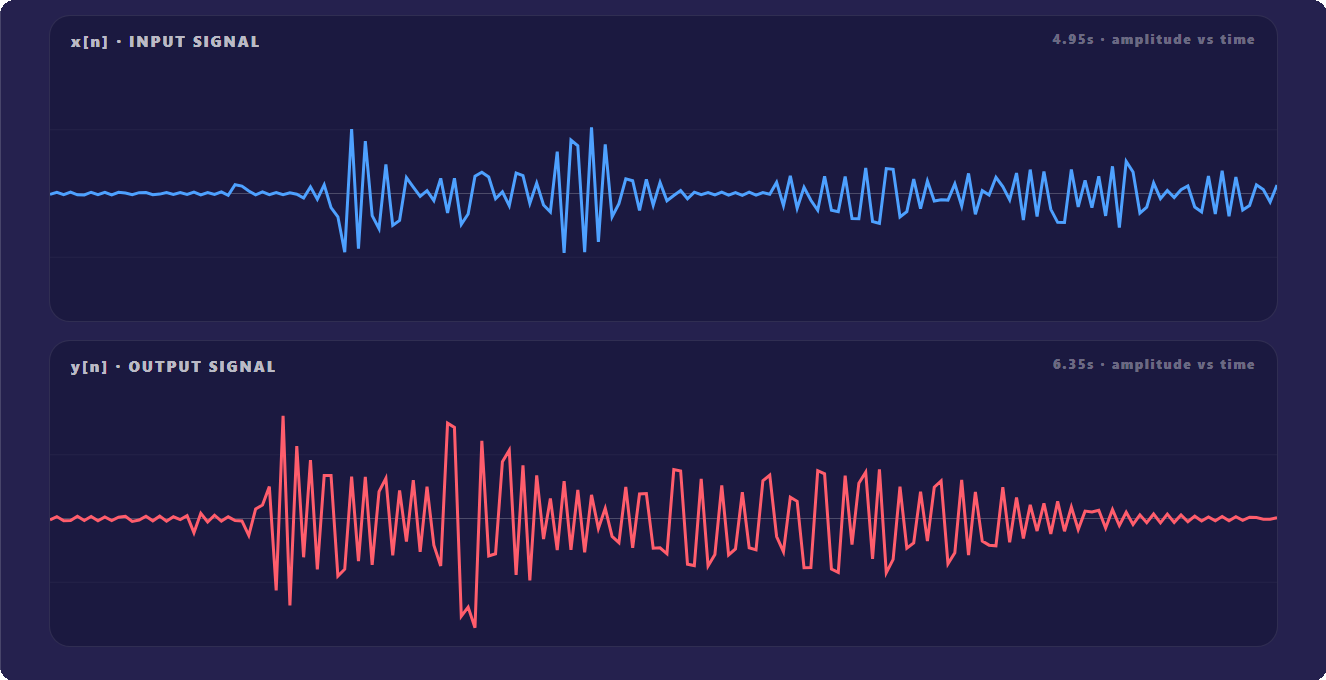
\includegraphics[width=0.85\linewidth]{amp_io.png}
  \caption{Input $x[n]$ (top) vs.\ output $y[n]$ (bottom) for a gain of $A=2$.}
\end{figure}

% ============================================================ 2. TIME-DOMAIN
\section{Time-Domain Processing}
This module covers three related effects --- Convolution, Echo, and
Delay --- that all operate directly on the raw sample stream
(``time domain'', as opposed to the frequency domain used later).

\subsection{Convolution}
\WhatHead
Convolution is the mathematical operation that describes how a signal
is reshaped by passing through any linear system --- for example, a
room's acoustics, which turns a sharp handclap into a long, blurred
decay (its \emph{impulse response}). Convolving a signal with a
recorded impulse response $h[n]$ makes the signal sound as if it was
played inside that room.

\AlgoHead
\begin{enumerate}
  \item Take the input signal $x[n]$ and an impulse response $h[n]$.
  \item \textbf{Reverse} $h$ in time, i.e.\ flip it back-to-front.
  \item \textbf{Slide} the reversed $h$ across $x$, one sample position
        at a time.
  \item At every position, \textbf{multiply} the overlapping samples of
        $x$ and the flipped/shifted $h$ pointwise, then \textbf{sum}
        all those products --- that single sum becomes one output
        sample $y[n]$.
  \item Repeat for every shift, from the moment the two signals first
        touch until the reversed $h$ has slid completely past $x$.
\end{enumerate}

\FormulaBox{$\displaystyle y[n] = \sum_{k} x[k]\,h[n-k]$}

\NoteHead
Computing this sum directly for every single output sample is
$O(N^2)$ and far too slow for a multi-second audio clip. The backend
instead computes it via \emph{FFT convolution}
(\texttt{scipy.signal.\allowbreak fftconvolve}): transform both signals to the
frequency domain, multiply their spectra pointwise, then transform
back. This is mathematically the exact same result, just computed in
$O(N\log N)$ time. The on-screen animation, however, plays out the
literal reverse-slide-multiply-accumulate definition above (on a
reduced number of points, so it stays watchable) so the algorithm
itself is visible, not just its output.

\begin{figure}[h]
  \centering
  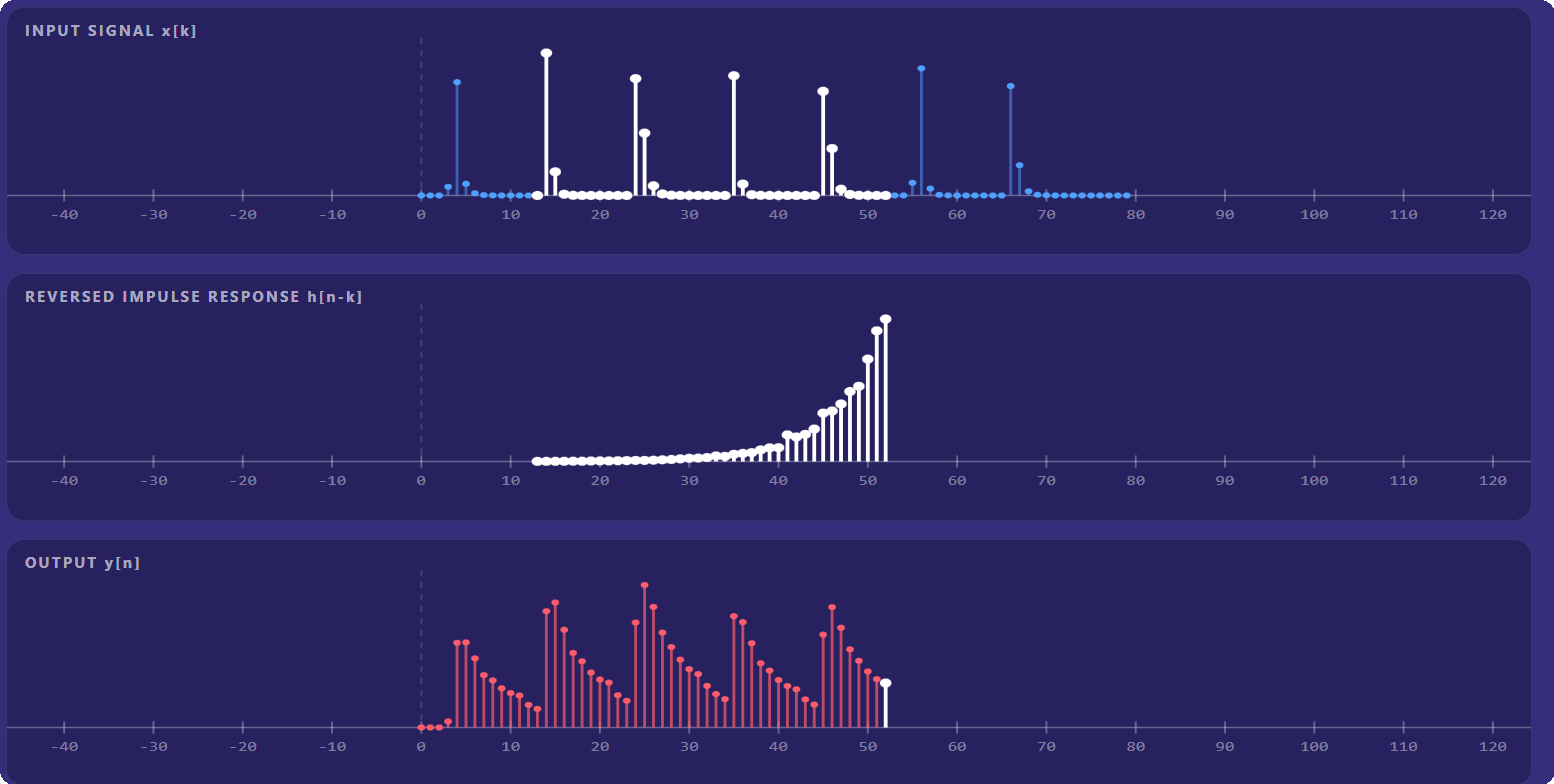
\includegraphics[width=0.9\linewidth]{conv_viz.png}
  \caption{The input $x[k]$, the reversed impulse response $h[n-k]$
  sliding across it, and the accumulating output $y[n]$.}
\end{figure}

\subsection{Echo}
\WhatHead
Echo layers several decaying, evenly-spaced repeats of the signal on
top of itself --- like shouting in a canyon and hearing your voice
come back multiple times, each time a little quieter.

\AlgoHead
\begin{enumerate}
  \item Start with the original (``dry'') signal as the base of the output.
  \item Make a copy of the signal delayed later in time by $D$ samples.
  \item Scale that delayed copy down by a decay factor $\alpha$ (where
        $0<\alpha<1$) and add it into the output.
  \item \textbf{Feed that result back} and repeat steps 2--3 a total of
        $R$ times: each new repeat is delayed by another $D$ samples
        and decayed by another factor of $\alpha$, so the $r$-th
        repeat is scaled by $\alpha^{r}$.
  \item The final output is the sum of the dry signal and all $R$
        decaying, delayed copies.
\end{enumerate}

\FormulaBox{$\displaystyle y[n]=x[n]+\sum_{r=1}^{R}\alpha^{r}\,x[n-rD]$}

\begin{figure}[h]
  \centering
  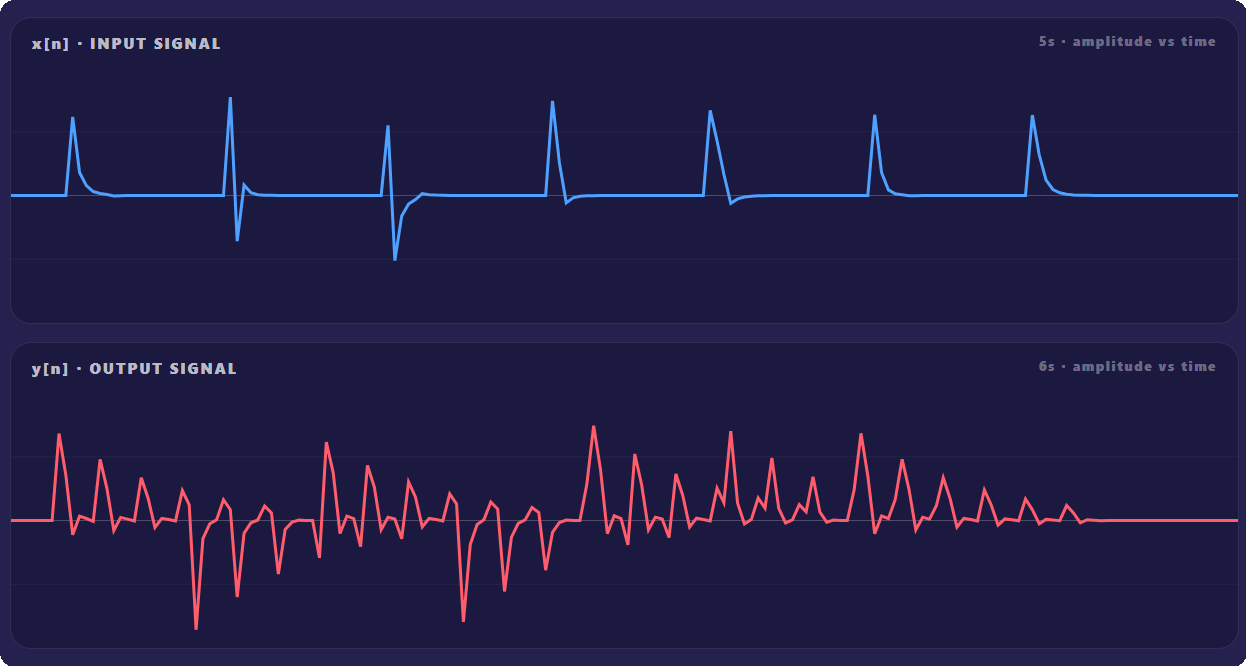
\includegraphics[width=0.75\linewidth]{echo_io.png}
  \caption{Input $x[n]$ vs.\ output $y[n]$ --- notice the repeated,
  progressively quieter reflections after each original spike.}
\end{figure}

\subsection{Delay}
\WhatHead
Delay is the simpler cousin of Echo: instead of a chain of repeats, it
adds back exactly \emph{one} clean, delayed copy of the signal --- no
feedback loop.

\AlgoHead
\begin{enumerate}
  \item Start with the original (dry) signal.
  \item Make \textbf{one} copy of the signal, delayed by $D$ samples.
        This copy is never fed back into itself the way Echo's is.
  \item Scale that single copy by a wet-mix factor $\alpha$.
  \item Add it to the original signal.
\end{enumerate}

\FormulaBox{$y[n]=x[n]+\alpha\cdot x[n-D]$}

\noindent Both effects use the exact same building block --- a scaled,
time-shifted copy $\alpha\,x[n-D]$ --- Echo simply applies it
recursively $R$ times, while Delay applies it exactly once.

\begin{figure}[h]
  \centering
  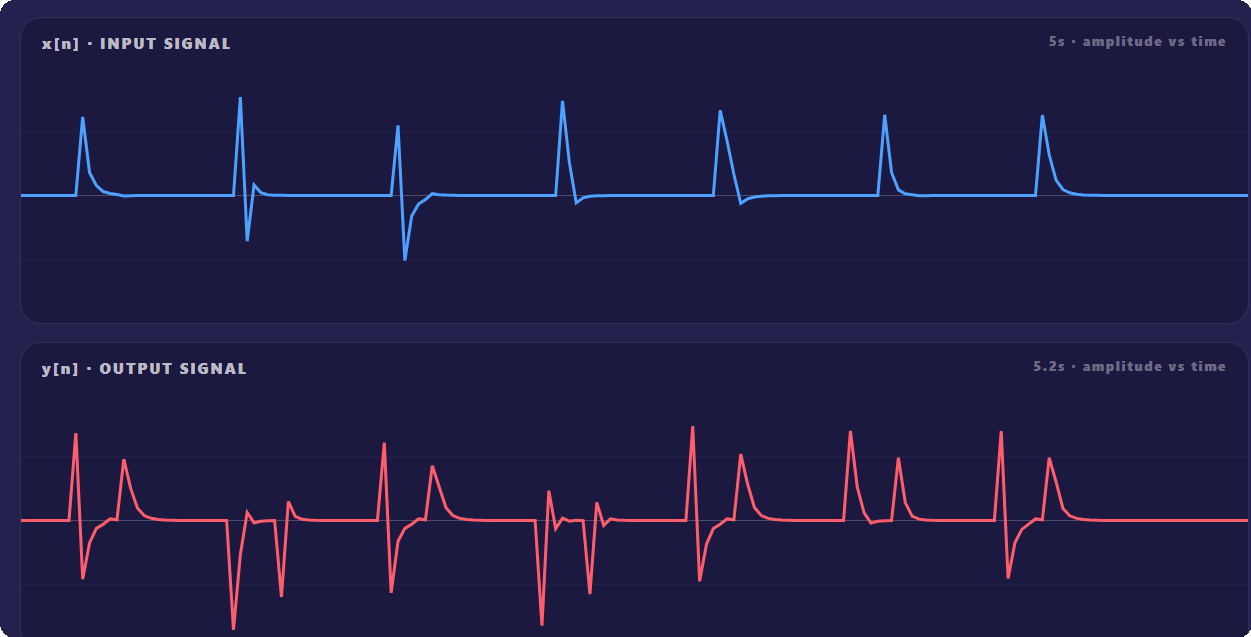
\includegraphics[width=0.75\linewidth]{delay_io.png}
  \caption{Input $x[n]$ vs.\ output $y[n]$ --- a single, clean, delayed repeat.}
\end{figure}

% ============================================================ 3. SPECTRAL DETECTION
\section{Spectral Detection --- Pitch}
\WhatHead
This module estimates the \emph{dominant pitch} of a signal --- the
strongest musical note present --- by looking at its frequency
content rather than its raw waveform, then synthesizes a pure tone at
that frequency so the detection can be verified by ear.

\AlgoHead
\begin{enumerate}
  \item Apply a Hann window to the signal (tapering its edges to zero)
        to reduce spectral leakage before transforming it.
  \item Compute the \textbf{FFT} of the windowed signal, giving the
        magnitude spectrum $|X(f)|$: how much energy exists at every
        frequency.
  \item Restrict the search to a user-chosen range $[f_{\min},
        f_{\max}]$, so DC offset, sub-bass rumble, and inaudible
        ultrasonic content cannot accidentally win.
  \item Find the frequency bin with the \textbf{largest magnitude}
        inside that range --- this is the detected dominant frequency
        $f_0$.
  \item Convert $f_0$ to the nearest musical note name using the
        standard equal-temperament formula (A4 $=$ 440\,Hz).
  \item \textbf{Synthesize} a short, pure sine wave at exactly $f_0$,
        so the answer can be checked by listening to it alongside the
        original.
\end{enumerate}

\FormulaBox{$f_0=\displaystyle\operatorname*{arg\,max}_{f\in[f_{\min},f_{\max}]}|X(f)| \qquad y[n]=A\sin(2\pi f_0 n/f_s)$}

\begin{figure}[h]
  \centering
  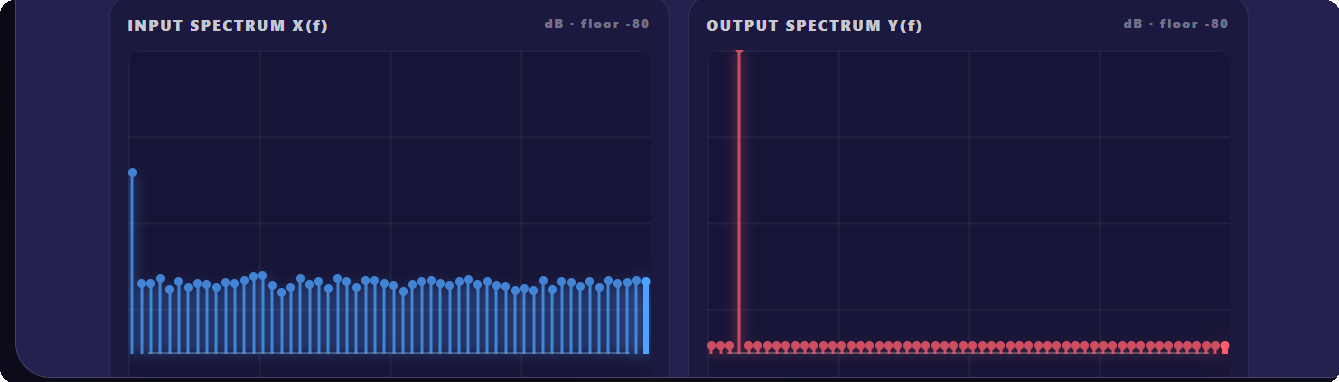
\includegraphics[width=0.95\linewidth]{pitch_spectra.png}
  \caption{Input spectrum $X(f)$ (left) --- energy spread across a
  fundamental and its overtones --- vs.\ the synthesized tone's
  spectrum $Y(f)$ (right), a single sharp spike exactly at $f_0$.}
\end{figure}

% ============================================================ 4. SAMPLING & QUANTIZATION
\section{Sampling \& Quantization}
This module demonstrates the two ways digitizing audio can lose
information: coarser \emph{amplitude} resolution (quantization) and
coarser \emph{time} resolution (sample-and-hold, a stand-in for a
lower sample rate).

\subsection{Quantization}
\WhatHead
A digital sample is stored using a fixed number of bits, which means
only a finite set of amplitude values is representable. Reducing that
bit depth forces every sample to snap to the nearest of a smaller set
of levels, which is audible as a gritty ``crunch'' called quantization
noise.

\AlgoHead
\begin{enumerate}
  \item Choose how many bits $b$ to keep (e.g.\ $4$ bits $=16$ levels).
  \item Compute the step size $\Delta$ that spans the full amplitude
        range $[-1,1]$ using $2^{b}$ evenly spaced levels.
  \item For every sample, divide by $\Delta$, \textbf{round} to the
        nearest whole number, then multiply back by $\Delta$ --- this
        snaps the sample onto the nearest allowed level.
  \item Clip the result to $[-1,1]$ to guarantee it stays in range.
\end{enumerate}

\FormulaBox{$y[n]=\Delta\cdot\mathrm{round}\!\left(\dfrac{x[n]}{\Delta}\right), \qquad \Delta = \dfrac{2}{2^{b}-1}$}

\subsection{Sample-and-Hold (Downsampling)}
\WhatHead
This simulates what happens when a signal is captured at a lower
sample rate: instead of measuring a fresh value at every time step,
the last measured value is simply \emph{held} until the next real
measurement arrives.

\AlgoHead
\begin{enumerate}
  \item Choose a hold factor $N$ --- the effective rate drops by a
        factor of $N$.
  \item Walk through the signal in consecutive blocks of $N$ samples.
  \item For each block, take the value of its \textbf{first} sample
        and repeat (hold) that same value for every position in the
        block, instead of reading a new value each time. This is
        exactly what a zero-order-hold DAC does.
\end{enumerate}

\FormulaBox{$y[n] = x\!\left(N\left\lfloor n/N\right\rfloor\right)$}

\noindent The output stays the same length as the input (each held
sample simply repeats $N$ times), producing a ``staircase'' shape.
This staircase is precisely what makes aliasing audible --- the
abrupt jumps introduce high-frequency energy that was never in the
original signal.

\begin{figure}[h]
  \centering
  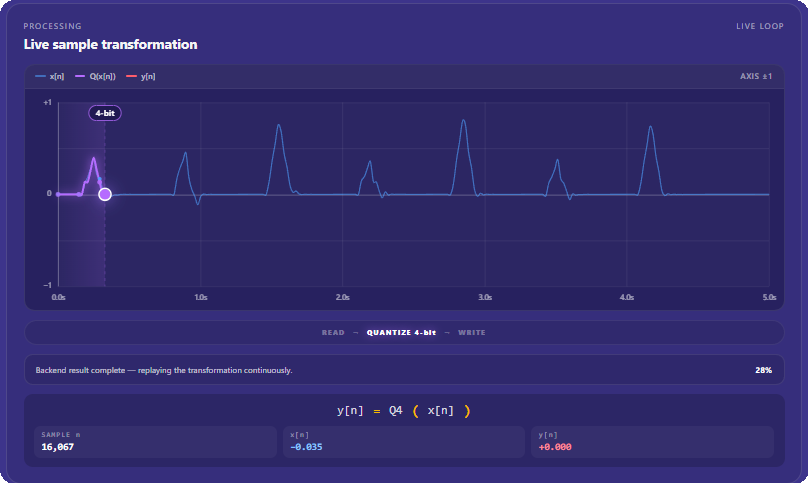
\includegraphics[width=0.46\linewidth]{quant_mid.png}\hfill
  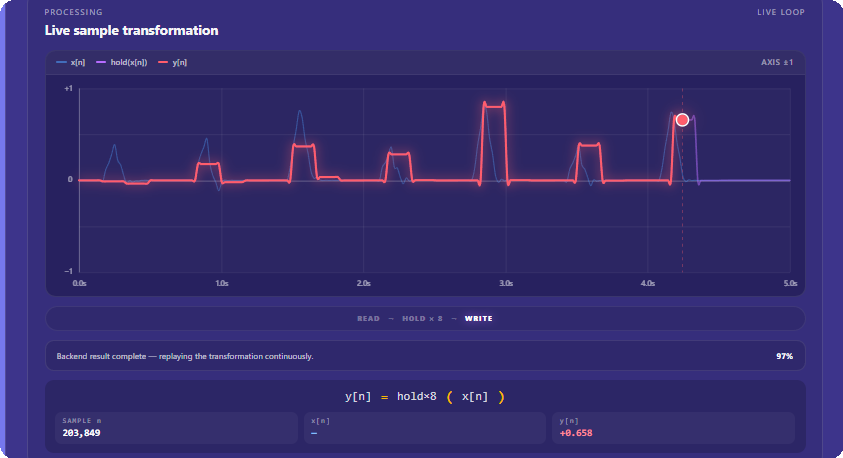
\includegraphics[width=0.46\linewidth]{sample_mid.png}
  \caption{Live transformation panels: quantization to 4-bit (left)
  and sample-and-hold at $\times 8$ (right). Both show the formula
  applied to the current sample in real time.}
\end{figure}

% ============================================================ 5. FILTERING
\section{Frequency \& Filtering}
\WhatHead
A digital filter reshapes a signal's frequency content --- e.g.\
removing everything above a cutoff frequency (lowpass) or everything
outside a band (bandpass). This module lets you design filters from
five classical IIR families (Butterworth, Chebyshev~I, Chebyshev~II,
Elliptic, Bessel) plus an ``ideal'' brick-wall filter, at four band
types (lowpass, highpass, bandpass, bandstop).

\AlgoHead
\begin{enumerate}
  \item Choose a filter family, a band type, cutoff frequency (or
        frequencies for band filters), and a filter order $N$ (higher
        order $=$ steeper roll-off, closer to an ideal brick wall).
  \item \textbf{Design the filter} using that family's standard design
        equations, producing the filter as \textbf{SOS} ---
        \emph{second-order sections}.
  \item \textbf{Apply the filter} to the signal using
        \texttt{sosfiltfilt}: run the SOS cascade across the signal
        once forwards, then once more backwards (on the
        time-reversed result).
\end{enumerate}

\FormulaBox{$Y(f) = X(f)\cdot H(f)$}

\subsection*{What is SOS, and why filter twice?}
A digital IIR filter is normally described by a transfer function ---
one set of numerator/denominator coefficients. For a high order (say,
8th order) or a very narrow band, those coefficients can span an
enormous numeric range, and ordinary floating-point rounding error in
that form is severe enough to make the filter numerically unstable ---
in the worst case, the output becomes entirely \texttt{NaN}.

\textbf{Second-order sections (SOS)} solve this by never building that
one giant filter at all. Instead, the design is expressed as a
\emph{cascade} (a chain) of many small, simple 2-pole/2-zero
(``biquad'') filter stages, each one individually well-conditioned,
multiplied together to form the overall response. Filtering the
signal through the small stages one after another gives the identical
mathematical result as the single high-order filter would, but stays
numerically stable at any order.

Running the SOS cascade only \emph{forwards} would also shift the
signal in time (phase distortion) --- later frequencies would lag
behind earlier ones. \texttt{sosfiltfilt} fixes this by filtering the
signal once forwards and once more backwards (i.e.\ filtering the
time-reversed signal, then reversing the result back). The delay
introduced by the forward pass is exactly cancelled by the backward
pass, so the final output lines up in time with the input perfectly
--- this is called \emph{zero-phase filtering}. The cost is that the
signal is effectively filtered twice (squaring the magnitude
response), which the design step already accounts for.

The one exception is the \textbf{``ideal'' family}: instead of
designing any IIR filter at all, it takes the FFT of the signal,
zeroes out every frequency bin outside the desired band directly, and
inverse-FFTs back --- a perfect brick-wall cutoff with no
transition band, used here mainly as a textbook comparison against the
real, imperfect filter families.

\begin{figure}[h]
  \centering
  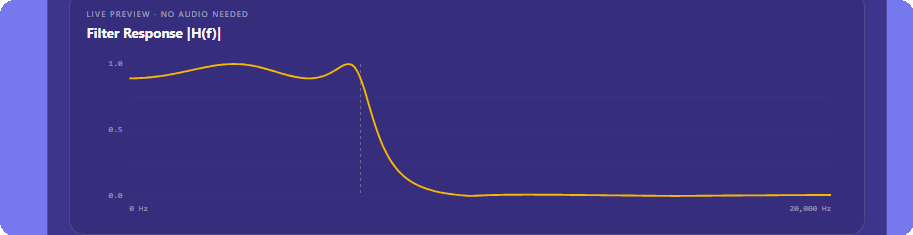
\includegraphics[width=0.85\linewidth]{filter_response.png}
  \caption{The filter's own frequency response $|H(f)|$ for a
  lowpass Butterworth design --- flat in the passband, then rolling
  off past the cutoff $f_c$.}
\end{figure}

% ============================================================ 6. VOICE MORPHING
\section{Voice Morphing --- Phase Vocoder}
\WhatHead
Every frequency-domain bin of a signal has two independent pieces of
information: a \textbf{magnitude} $|X(f)|$ (how much energy is at that
frequency) and a \textbf{phase} $\angle X(f)$ (that frequency
component's timing/alignment). This module manipulates those two
pieces \emph{independently} to produce four different effects.

\FormulaBox{$X(f)=|X(f)|\cdot e^{\,j\angle X(f)}$}

\subsection{Pitch Shift \& Time Stretch --- the Phase Vocoder}
Pitch-shifting and time-stretching both rely on the same underlying
engine, called a \emph{phase vocoder}. Time-stretching changes how
long the signal lasts while keeping every frequency exactly where it
was; pitch-shifting reuses that same time-stretch and then resamples
the result to restore the original duration, which moves the pitch.

\AlgoHead
\begin{enumerate}
  \item \textbf{STFT}: split the audio into overlapping windowed
        frames and FFT each one, analyzing magnitude and phase of
        every bin \emph{separately} for every frame.
  \item \textbf{Time-mapping}: decide new frame positions for the
        desired stretch rate $r$. The output (synthesis) frames stay
        evenly spaced as usual, but the corresponding input (analysis)
        read-position advances by $r$ times the normal spacing --- so
        for $r<1$ frames are read more densely (stretching the sound
        out), and for $r>1$ more sparsely (compressing it). This
        desired read-position is usually a fractional index, landing
        \emph{between} two frames that were actually computed.
  \item \textbf{Magnitude interpolation}: since the desired analysis
        position falls between two real frames, linearly interpolate
        the magnitude spectra of those two neighboring frames to
        estimate the magnitude at the in-between position.
  \item \textbf{Phase updating}: phase cannot simply be interpolated
        the same way --- doing so produces a smeared, ``phasy'' sound.
        Instead, for each frequency bin, the algorithm measures how
        much the phase actually advanced between consecutive analysis
        frames, uses that to estimate the bin's \emph{true
        instantaneous frequency}, and then \emph{accumulates}
        (integrates) the phase forward from the previous synthesis
        frame using that true frequency, at the new synthesis hop
        spacing. This keeps the phase relationships between frames
        coherent across the whole clip --- it is the specific trick
        that makes a phase vocoder work, and the reason it isn't
        called just a ``magnitude vocoder''.
  \item \textbf{Reconstruct}: combine the interpolated magnitude with
        the newly accumulated phase into a new complex spectrum per
        frame, inverse-FFT each frame, and overlap-add the frames back
        into one continuous time-domain signal. At this point the
        signal's \emph{duration} has changed by the stretch ratio, but
        every frequency is still where it started.
  \item \textbf{Pitch shift only}: take that time-stretched result and
        \textbf{resample} it back to the original sample count.
        Resampling changes the playback rate, which shifts every
        frequency proportionally --- undoing the duration change while
        leaving the pitch shifted. Net effect: only the pitch moves;
        the duration returns to exactly what it was.
\end{enumerate}

\subsection{Robot (Zero Phase) and Whisper (Random Phase)}
\WhatHead
These two effects skip the whole time-mapping/interpolation machinery
above --- they take a single STFT of the whole clip and only rewrite
its phase, leaving every magnitude value completely untouched.

\AlgoHead
\begin{enumerate}
  \item Take one STFT of the signal, obtaining magnitude $|X(f)|$ and
        phase $\angle X(f)$ for every bin of every frame.
  \item \textbf{Robot}: set every bin's phase to exactly $0$, keeping
        magnitude unchanged. \textbf{Whisper}: replace every bin's
        phase with an independent random value instead, also keeping
        magnitude unchanged.
  \item Inverse-STFT the result back into audio.
\end{enumerate}

\FormulaBox{\textbf{Robot:}\; $Y(f)=|X(f)|\cdot e^{j\cdot 0}=|X(f)|\qquad$ \textbf{Whisper:}\; $Y(f)=|X(f)|\cdot e^{j\theta},\ \theta\sim\text{random}$}

\noindent Since \emph{nothing} about $|X(f)|$ changes in either case,
these effects are direct proof that phase --- not magnitude --- carries
a voice's sense of timing and ``voicedness''. Zeroing phase collapses
every frequency component to start at the same instant, producing a
flat, buzzy monotone (Robot). Randomizing phase instead decorrelates
the components without collapsing them, producing a breathy,
unvoiced, whisper-like texture.

Named presets (\emph{Vader-style}, \emph{Protocol Droid}, \emph{Radio
Trooper}, \emph{Cylon Monotone}) start from this same zero-phase Robot
base and layer additional, already-covered effects on top of it ---
pitch shifting, lowpass/bandpass filtering, soft-clip distortion, ring
modulation, and reverb --- to build more specific character voices.

\begin{figure}[h]
  \centering
  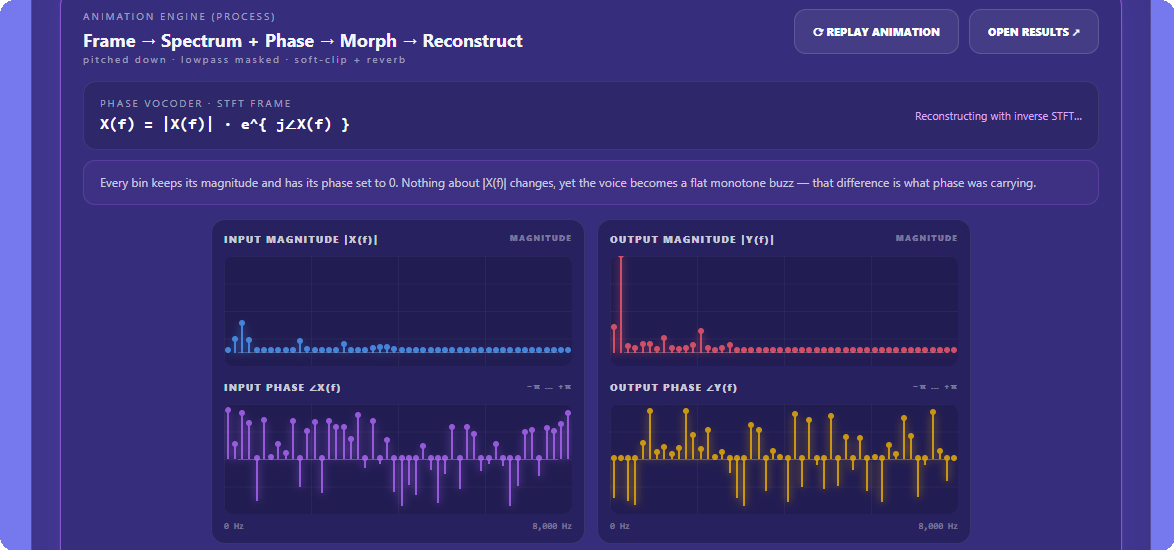
\includegraphics[width=0.9\linewidth]{morph_panels.png}
  \caption{Robot mode: input magnitude/phase (left) vs.\ output
  magnitude/phase (right). Magnitude is unchanged; the scattered input
  phase has been flattened to zero.}
\end{figure}

% ============================================================ 7. SPECTRAL PORTAL
\section{Spectral Portal --- Spectrogram Masking}
\WhatHead
This module lets you literally paint on a picture of the sound's
frequency content over time, erasing or isolating whichever
time-frequency regions you select --- for example, removing a specific
tone that only happens between 1 and 3 seconds, without touching
anything else.

\AlgoHead
\begin{enumerate}
  \item \textbf{Build the spectrogram}: split the signal into
        overlapping windowed frames and FFT each one (an STFT), giving
        a 2-D grid where the horizontal axis is time, the vertical
        axis is frequency, and each cell's value is $|X(k,m)|$ in
        decibels for frequency bin $k$ and time frame $m$.
  \item \textbf{Colour the grid} on a purple-to-gold scale, normalized
        between that clip's own quietest and loudest cell --- quiet
        cells render dark purple, loud cells render bright gold.
  \item \textbf{Paint KEEP or ERASE rectangles} directly on that image,
        in real Hz/second coordinates.
  \item \textbf{Build a mask} $M(k,m)$ from those rectangles: if any
        ``keep'' region was drawn, everything starts silent
        ($M=0$) and only the keep regions are set to $1$ (an isolating
        mask); otherwise everything starts audible ($M=1$) and only the
        erase regions are set to $0$ (a subtractive mask). Later
        regions win where two overlap, matching paint order.
  \item \textbf{Feather the mask}: apply a Gaussian blur across both
        axes of the mask before using it. A hard rectangular cut would
        create sharp discontinuities in the spectrum, which the
        inverse transform would hear as ringing/``musical noise'';
        blurring softens every edge into a smooth ramp instead.
  \item \textbf{Apply the mask}: multiply the mask elementwise into the
        complex STFT, $X'(k,m)=M(k,m)\cdot X(k,m)$.
  \item \textbf{Inverse STFT} (with overlap-add) reconstructs the
        edited time-domain audio from what remains of the spectrum.
\end{enumerate}

\FormulaBox{$X'(k,m)=M(k,m)\cdot X(k,m)$}

\begin{figure}[h]
  \centering
  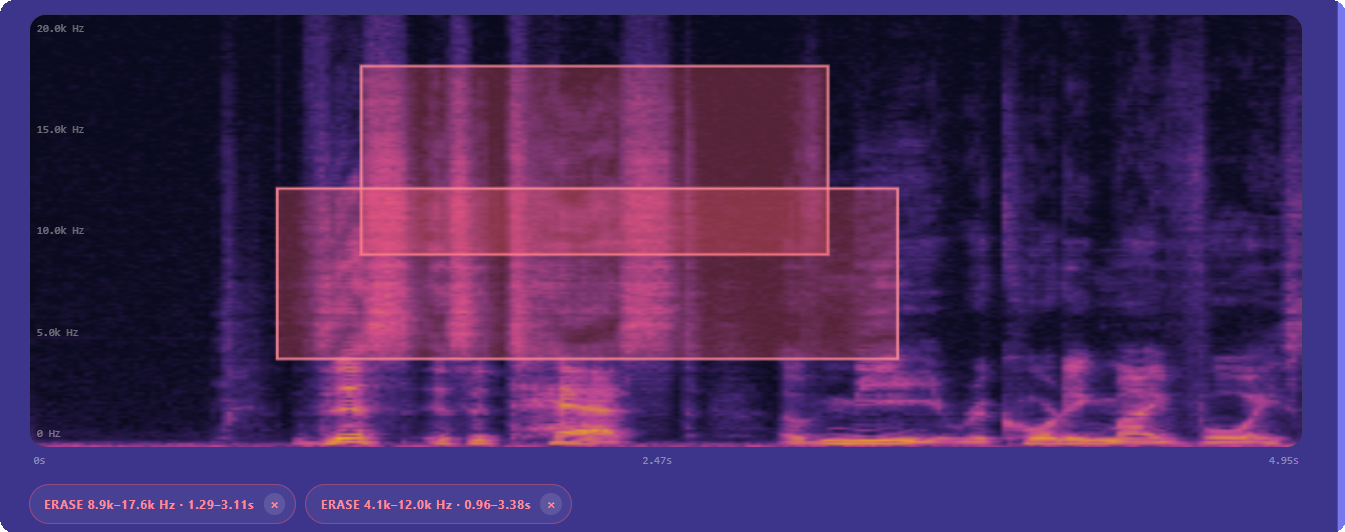
\includegraphics[width=0.85\linewidth]{spectrogram_mask.png}\\[0.4em]
  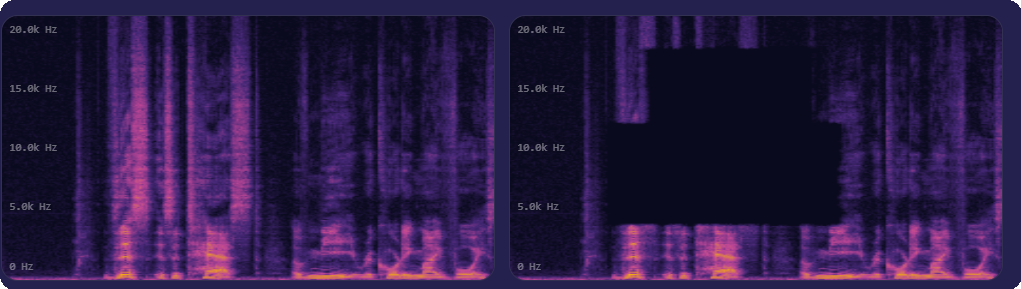
\includegraphics[width=0.65\linewidth]{spectrogram_before_after.png}
  \caption{Top: two erase regions drawn on the spectrogram, with their
  Hz/time bounds. Bottom: the resulting spectrogram before (left) and
  after (right) the mask is applied --- the erased region is now silent.}
\end{figure}

% ============================================================ STUDIO
\section{Studio --- Multi-Operation Signal Chain}
\WhatHead
The Studio page lets any of the effects above be composed into one
ordered pipeline, so complex processing chains (e.g.\ filter $\to$
amplify $\to$ reverb) can be built and run as a single job.

\AlgoHead
\begin{enumerate}
  \item Upload or record one input signal, used as the chain's starting point.
  \item Add operation steps to the chain, in any order (up to 25 steps), each with its own parameters.
  \item Run the chain: the backend executes each step in sequence,
        and \textbf{every step's output becomes the next step's
        input}.
  \item Each step reports its own elapsed time and signal
        levels, and the final result is added to a comparison history
        so different chains/parameters can be judged side by side.
\end{enumerate}

\FormulaBox{$y[n]=f_K\!\big(f_{K-1}(\cdots f_1(x[n])\cdots)\big)$}

\noindent where $f_1,\dots,f_K$ are the chain's steps in order, and
each $f_i$ is exactly one of the algorithms described in the sections
above.

% ============================================================ CONCLUSION
\section{Technology Summary}
\begin{itemize}[leftmargin=1.4em]
  \item \textbf{Backend engine:} Python, FastAPI, NumPy, SciPy, Librosa, soundfile.
  \item \textbf{Frontend interaction:} React, Vite, Canvas-based live visualizations.
  \item \textbf{DSP methods covered:} FFT \& spectrograms, convolution,
        IIR filtering with SOS/zero-phase filtering, quantization \&
        aliasing, the phase vocoder, and frequency-domain masking.
\end{itemize}

\vspace{1em}
\noindent Every module above is computed for real on the backend from
the audio you provide --- the figures in this document are actual
screenshots of the application's own output, not illustrations.

\end{document}
